\chapter{Planejamento}

Conforme descrito no Capítulo \ref{cap:introducao}, este trabalho será constituído de cinco etapas.
Em um primeiro momento, a etapa de diagnóstico foi realizada e os sistemas relacionados e suas funcionalidades em comum foram apresentadas no Capítulo \ref{cap:sistemas_relacionados}.

Na Tabela \ref{tab:principais_funcionalidades} são apresentadas as principais funcionalidades em comum encontradas nos sistemas, de acordo com as categorias previamente estabelecidas.

\begin{table}[ht!]
\centering
\caption{Funcionalidades encontradas nos sistemas relacionados}
\label{tab:principais_funcionalidades}
\begin{tabular}{l|l}
\hline
\multicolumn{1}{c|}{\textbf{Categoria}} & \multicolumn{1}{c}{\textbf{Funcionalidades}} \\ \hline
\begin{tabular}[c]{@{}l@{}} Levantamento de Dados\\ e estatísticas\end{tabular} & \begin{tabular}[c]{@{}l@{}} - Categorização e junção dos dados obtidos de cada mulher \\ (através de questionário ou formulário de denúncia)\end{tabular} \\ \hline 
Mapeamento de Riscos & \begin{tabular}[c]{@{}l@{}}-  Mapeamento de locais de riscos por meio das denúncias de \\ violência realizadas\end{tabular} \\ \hline
Informativos & \begin{tabular}[c]{@{}l@{}} - Disponibilização de leis e conceitos relacionados \\ - Auxílio na descoberta da violência sofrida \\ - Disponibilização de notícias\end{tabular}  \\ \hline
Pedidos de Socorro & - Envio de pedido de socorro às autoridades competentes \\ \hline
Denúncia & \begin{tabular}[c]{@{}l@{}}- Denúncia da violência sofrida às autoridades competentes\\ - Compartilhamento da
violência sofrida para: \\ \hspace{1em} - alerta à outras mulheres \\ \hspace{1em} - levantamento de dados \end{tabular} \\ \hline
\end{tabular}
\end{table}

\section{Escopo da API}

Considerando as funcionalidades em comum encontradas e as funcionalidades providas pelo I-DECIDE, 
o escopo a ser implementado na API é o armazenamento e fornecimento de:

\begin{itemize}
	\item Dados de denúncias;
	\item Estatísticas de acordo com estes dados;
	\item Tipos de violência;
	\item Questões para descoberta do tipo de violência sofrida;
	\item Ações para sair da situação de violência de forma segura;
	\item Questões para geração do plano de segurança;
\end{itemize}


\subsection{Estrutura da API}

De acordo com o escopo definido, definiu-se a estrutura da API apresentada na Figura \ref{fig:estrutura_api}.

\begin{figure}[h!]
\centering
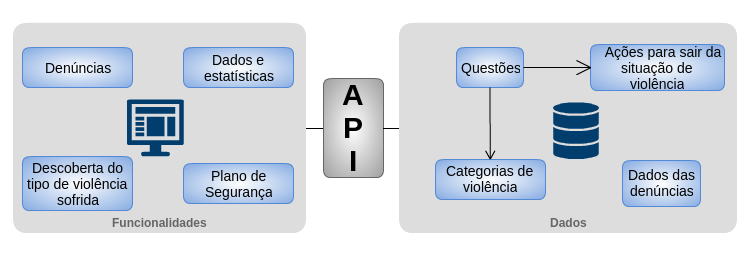
\includegraphics[scale=0.7]{figuras/estrutura_api.png}
\caption{Estrutura da API}
\label{fig:estrutura_api}
\end{figure}

A API será implementada utilizando a arquitetura REST, o framework Django Rest Framework e a linguagem Python.

\section{Cronograma}

Para execução do trabalho foi estabelecido um cronograma que pode ser visto na Figura \ref{fig:cronograma}.

\begin{figure}[h!]
\centering
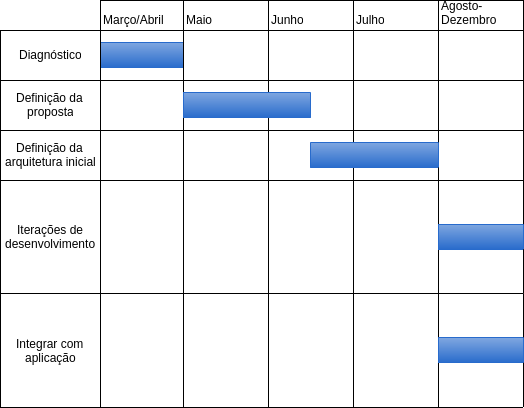
\includegraphics[scale=0.8]{figuras/cronograma.png}
\caption{Cronograma de execução}
\label{fig:cronograma}
\end{figure}

